% Created by tikzDevice version 0.12.6 on 2026-06-07 17:42:47
% !TEX encoding = UTF-8 Unicode
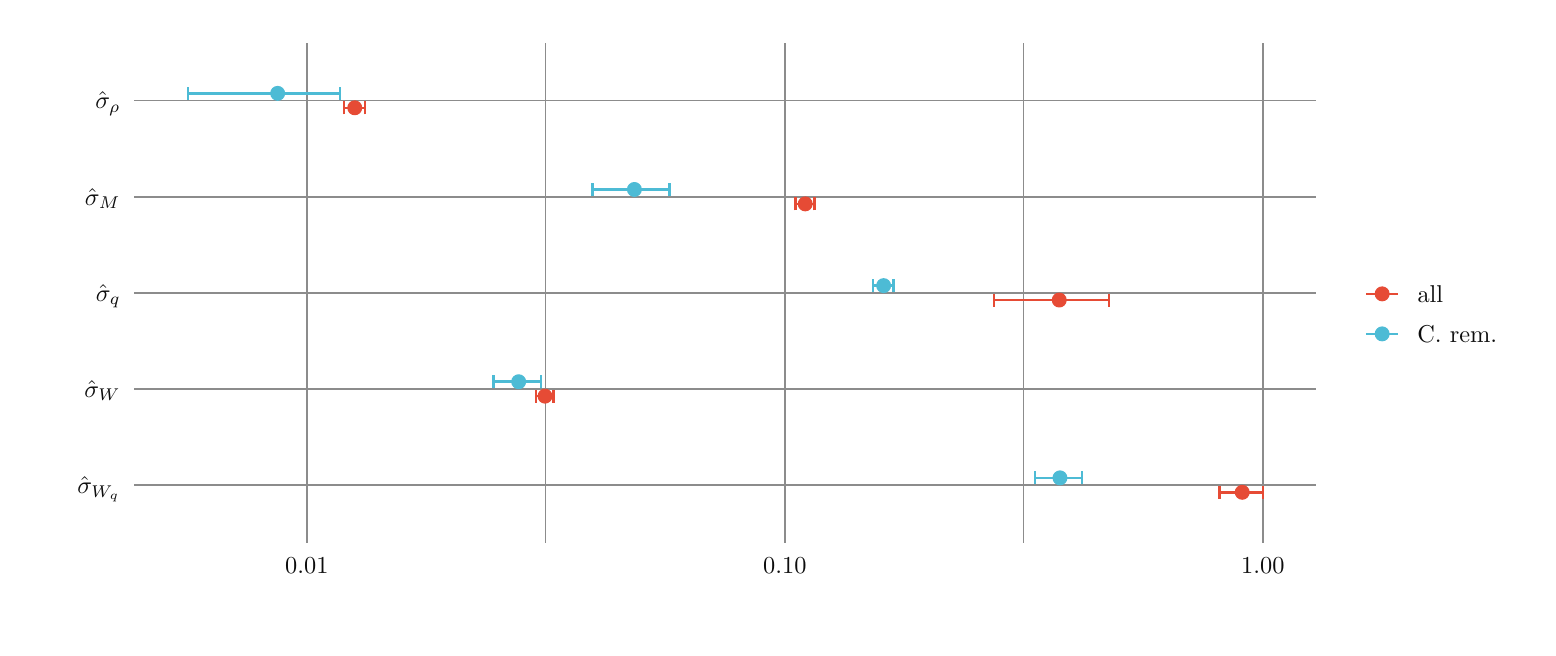
\begin{tikzpicture}[x=1pt,y=1pt]
\definecolor{fillColor}{RGB}{255,255,255}
\path[use as bounding box,fill=fillColor,fill opacity=0.00] (0,0) rectangle (542.02,216.81);
\begin{scope}
\path[clip] ( 38.50, 30.69) rectangle (465.71,211.31);
\definecolor{drawColor}{gray}{0.55}

\path[draw=drawColor,line width= 0.3pt,line join=round] (187.23, 30.69) --
	(187.23,211.31);

\path[draw=drawColor,line width= 0.3pt,line join=round] (359.95, 30.69) --
	(359.95,211.31);

\path[draw=drawColor,line width= 0.6pt,line join=round] ( 38.50, 51.53) --
	(465.71, 51.53);

\path[draw=drawColor,line width= 0.6pt,line join=round] ( 38.50, 86.26) --
	(465.71, 86.26);

\path[draw=drawColor,line width= 0.6pt,line join=round] ( 38.50,121.00) --
	(465.71,121.00);

\path[draw=drawColor,line width= 0.6pt,line join=round] ( 38.50,155.73) --
	(465.71,155.73);

\path[draw=drawColor,line width= 0.6pt,line join=round] ( 38.50,190.47) --
	(465.71,190.47);

\path[draw=drawColor,line width= 0.6pt,line join=round] (100.87, 30.69) --
	(100.87,211.31);

\path[draw=drawColor,line width= 0.6pt,line join=round] (273.59, 30.69) --
	(273.59,211.31);

\path[draw=drawColor,line width= 0.6pt,line join=round] (446.31, 30.69) --
	(446.31,211.31);
\definecolor{drawColor}{RGB}{230,75,53}
\definecolor{fillColor}{RGB}{230,75,53}

\path[draw=drawColor,line width= 0.4pt,line join=round,line cap=round,fill=fillColor] (438.87, 48.92) circle (  2.50);
\definecolor{drawColor}{RGB}{77,187,213}
\definecolor{fillColor}{RGB}{77,187,213}

\path[draw=drawColor,line width= 0.4pt,line join=round,line cap=round,fill=fillColor] (373.01, 54.13) circle (  2.50);
\definecolor{drawColor}{RGB}{230,75,53}
\definecolor{fillColor}{RGB}{230,75,53}

\path[draw=drawColor,line width= 0.4pt,line join=round,line cap=round,fill=fillColor] (186.94, 83.66) circle (  2.50);
\definecolor{drawColor}{RGB}{77,187,213}
\definecolor{fillColor}{RGB}{77,187,213}

\path[draw=drawColor,line width= 0.4pt,line join=round,line cap=round,fill=fillColor] (177.42, 88.87) circle (  2.50);
\definecolor{drawColor}{RGB}{230,75,53}
\definecolor{fillColor}{RGB}{230,75,53}

\path[draw=drawColor,line width= 0.4pt,line join=round,line cap=round,fill=fillColor] (372.76,118.39) circle (  2.50);
\definecolor{drawColor}{RGB}{77,187,213}
\definecolor{fillColor}{RGB}{77,187,213}

\path[draw=drawColor,line width= 0.4pt,line join=round,line cap=round,fill=fillColor] (309.30,123.60) circle (  2.50);
\definecolor{drawColor}{RGB}{230,75,53}
\definecolor{fillColor}{RGB}{230,75,53}

\path[draw=drawColor,line width= 0.4pt,line join=round,line cap=round,fill=fillColor] (280.97,153.13) circle (  2.50);
\definecolor{drawColor}{RGB}{77,187,213}
\definecolor{fillColor}{RGB}{77,187,213}

\path[draw=drawColor,line width= 0.4pt,line join=round,line cap=round,fill=fillColor] (219.24,158.34) circle (  2.50);
\definecolor{drawColor}{RGB}{230,75,53}
\definecolor{fillColor}{RGB}{230,75,53}

\path[draw=drawColor,line width= 0.4pt,line join=round,line cap=round,fill=fillColor] (118.19,187.86) circle (  2.50);
\definecolor{drawColor}{RGB}{77,187,213}
\definecolor{fillColor}{RGB}{77,187,213}

\path[draw=drawColor,line width= 0.4pt,line join=round,line cap=round,fill=fillColor] ( 90.33,193.07) circle (  2.50);
\definecolor{drawColor}{RGB}{230,75,53}

\path[draw=drawColor,line width= 0.9pt,line join=round] (446.29, 46.58) --
	(446.29, 51.27);

\path[draw=drawColor,line width= 0.9pt,line join=round] (446.29, 48.92) --
	(430.63, 48.92);

\path[draw=drawColor,line width= 0.9pt,line join=round] (430.63, 46.58) --
	(430.63, 51.27);
\definecolor{drawColor}{RGB}{77,187,213}

\path[draw=drawColor,line width= 0.9pt,line join=round] (381.04, 51.79) --
	(381.04, 56.48);

\path[draw=drawColor,line width= 0.9pt,line join=round] (381.04, 54.13) --
	(364.01, 54.13);

\path[draw=drawColor,line width= 0.9pt,line join=round] (364.01, 51.79) --
	(364.01, 56.48);
\definecolor{drawColor}{RGB}{230,75,53}

\path[draw=drawColor,line width= 0.9pt,line join=round] (190.08, 81.31) --
	(190.08, 86.00);

\path[draw=drawColor,line width= 0.9pt,line join=round] (190.08, 83.66) --
	(183.66, 83.66);

\path[draw=drawColor,line width= 0.9pt,line join=round] (183.66, 81.31) --
	(183.66, 86.00);
\definecolor{drawColor}{RGB}{77,187,213}

\path[draw=drawColor,line width= 0.9pt,line join=round] (185.47, 86.52) --
	(185.47, 91.21);

\path[draw=drawColor,line width= 0.9pt,line join=round] (185.47, 88.87) --
	(168.40, 88.87);

\path[draw=drawColor,line width= 0.9pt,line join=round] (168.40, 86.52) --
	(168.40, 91.21);
\definecolor{drawColor}{RGB}{230,75,53}

\path[draw=drawColor,line width= 0.9pt,line join=round] (390.67,116.05) --
	(390.67,120.74);

\path[draw=drawColor,line width= 0.9pt,line join=round] (390.67,118.39) --
	(349.17,118.39);

\path[draw=drawColor,line width= 0.9pt,line join=round] (349.17,116.05) --
	(349.17,120.74);
\definecolor{drawColor}{RGB}{77,187,213}

\path[draw=drawColor,line width= 0.9pt,line join=round] (312.91,121.26) --
	(312.91,125.95);

\path[draw=drawColor,line width= 0.9pt,line join=round] (312.91,123.60) --
	(305.50,123.60);

\path[draw=drawColor,line width= 0.9pt,line join=round] (305.50,121.26) --
	(305.50,125.95);
\definecolor{drawColor}{RGB}{230,75,53}

\path[draw=drawColor,line width= 0.9pt,line join=round] (284.30,150.78) --
	(284.30,155.47);

\path[draw=drawColor,line width= 0.9pt,line join=round] (284.30,153.13) --
	(277.49,153.13);

\path[draw=drawColor,line width= 0.9pt,line join=round] (277.49,150.78) --
	(277.49,155.47);
\definecolor{drawColor}{RGB}{77,187,213}

\path[draw=drawColor,line width= 0.9pt,line join=round] (231.86,155.99) --
	(231.86,160.68);

\path[draw=drawColor,line width= 0.9pt,line join=round] (231.86,158.34) --
	(204.07,158.34);

\path[draw=drawColor,line width= 0.9pt,line join=round] (204.07,155.99) --
	(204.07,160.68);
\definecolor{drawColor}{RGB}{230,75,53}

\path[draw=drawColor,line width= 0.9pt,line join=round] (121.89,185.52) --
	(121.89,190.21);

\path[draw=drawColor,line width= 0.9pt,line join=round] (121.89,187.86) --
	(114.30,187.86);

\path[draw=drawColor,line width= 0.9pt,line join=round] (114.30,185.52) --
	(114.30,190.21);
\definecolor{drawColor}{RGB}{77,187,213}

\path[draw=drawColor,line width= 0.9pt,line join=round] (112.89,190.73) --
	(112.89,195.42);

\path[draw=drawColor,line width= 0.9pt,line join=round] (112.89,193.07) --
	( 57.92,193.07);

\path[draw=drawColor,line width= 0.9pt,line join=round] ( 57.92,190.73) --
	( 57.92,195.42);
\end{scope}
\begin{scope}
\path[clip] (  0.00,  0.00) rectangle (542.02,216.81);
\definecolor{drawColor}{gray}{0.05}

\node[text=drawColor,anchor=base east,inner sep=0pt, outer sep=0pt, scale=  0.88] at ( 33.55, 48.50) {$\hat\sigma_{ W_q }$};

\node[text=drawColor,anchor=base east,inner sep=0pt, outer sep=0pt, scale=  0.88] at ( 33.55, 83.23) {$\hat\sigma_{ W }$};

\node[text=drawColor,anchor=base east,inner sep=0pt, outer sep=0pt, scale=  0.88] at ( 33.55,117.97) {$\hat\sigma_{ q }$};

\node[text=drawColor,anchor=base east,inner sep=0pt, outer sep=0pt, scale=  0.88] at ( 33.55,152.70) {$\hat\sigma_{ M }$};

\node[text=drawColor,anchor=base east,inner sep=0pt, outer sep=0pt, scale=  0.88] at ( 33.55,187.44) {$\hat\sigma_{ \rho }$};
\end{scope}
\begin{scope}
\path[clip] (  0.00,  0.00) rectangle (542.02,216.81);
\definecolor{drawColor}{gray}{0.05}

\node[text=drawColor,anchor=base,inner sep=0pt, outer sep=0pt, scale=  0.88] at (100.87, 19.68) {0.01};

\node[text=drawColor,anchor=base,inner sep=0pt, outer sep=0pt, scale=  0.88] at (273.59, 19.68) {0.10};

\node[text=drawColor,anchor=base,inner sep=0pt, outer sep=0pt, scale=  0.88] at (446.31, 19.68) {1.00};
\end{scope}
\begin{scope}
\path[clip] (  0.00,  0.00) rectangle (542.02,216.81);
\definecolor{drawColor}{RGB}{230,75,53}
\definecolor{fillColor}{RGB}{230,75,53}

\path[draw=drawColor,line width= 0.4pt,line join=round,line cap=round,fill=fillColor] (489.44,120.62) circle (  2.50);
\end{scope}
\begin{scope}
\path[clip] (  0.00,  0.00) rectangle (542.02,216.81);
\definecolor{drawColor}{RGB}{230,75,53}

\path[draw=drawColor,line width= 0.9pt,line join=round] (483.65,120.62) -- (495.22,120.62);
\end{scope}
\begin{scope}
\path[clip] (  0.00,  0.00) rectangle (542.02,216.81);
\definecolor{drawColor}{RGB}{77,187,213}
\definecolor{fillColor}{RGB}{77,187,213}

\path[draw=drawColor,line width= 0.4pt,line join=round,line cap=round,fill=fillColor] (489.44,106.16) circle (  2.50);
\end{scope}
\begin{scope}
\path[clip] (  0.00,  0.00) rectangle (542.02,216.81);
\definecolor{drawColor}{RGB}{77,187,213}

\path[draw=drawColor,line width= 0.9pt,line join=round] (483.65,106.16) -- (495.22,106.16);
\end{scope}
\begin{scope}
\path[clip] (  0.00,  0.00) rectangle (542.02,216.81);
\definecolor{drawColor}{gray}{0.05}

\node[text=drawColor,anchor=base west,inner sep=0pt, outer sep=0pt, scale=  0.88] at (502.16,117.59) {all};
\end{scope}
\begin{scope}
\path[clip] (  0.00,  0.00) rectangle (542.02,216.81);
\definecolor{drawColor}{gray}{0.05}

\node[text=drawColor,anchor=base west,inner sep=0pt, outer sep=0pt, scale=  0.88] at (502.16,103.13) {C. rem.};
\end{scope}
\end{tikzpicture}
